%-------------------------------------------------------------------------------
\chapter[Bedload sediment transport]{Bedload Transport}\label{sec:BedloadTransport}
%-------------------------------------------------------------------------------

%-------------------------------------------------------------------------------
\section{Preliminaries}
%-------------------------------------------------------------------------------
The term bedload describes particles in a flowing fluid (usually water) that are transported along the bed. Bedload moves by rolling, sliding, and/or saltating (hopping). An exhaustive analysis of this topic can be found in~\cite{GarciaBook2006} and references therein.\\

\sisyphe{} solves the conservative law equation for sediment mass or Exner equation:

\begin{align}
(1-\lambda)\frac{\partial z_b}{\partial t} + \nabla\cdot \mathbf Q_b = 0
\label{eq:Exner}
\end{align}
with $\mathbf Q_b$ the vector of volumetric transport rate per unit width without pores (m$^2/$s), with components $Q_{b_x}, Q_{b_y}$ in the $x$ and $y$ direction respectively, $z_b$ is the bottom elevation (m) and $\lambda$ the bed porosity. The bedload transport vector can be decomposed into $x-$ and $y-$direction components as:
\begin{align}
\mathbf Q_b = (Q_{b_x}, Q_{b_y}) = (Q_b \cos\alpha, Q_b \sin\alpha).
\label{eq:bedloadtransportvector}
\end{align}
Above, $Q_b$ is the bedload transport rate per unit width, computed as a function of the equilibrium sediment load closure (or sediment transport capacity) and $\alpha$ is the angle between the sediment transport vector and the downstream direction ($x-$axis).

The deviation of the bed load direction from the flow direction is mainly influenced by the bed slope and the presence of secondary flows~\cite{Talmon95}, see Section~\ref{sec:corrections}.

%...............................................................................
\section{Steering file setup for bedload transport}
%...............................................................................
Bedload sediment transport can be set with the keyword \telkey{BED LOAD = YES} (logical type variable, set to {\ttfamily = YES} by default).

The dimensionless current-induced sediment transport rate $\Phi_b$ is expressed by:
\begin{align}
\Phi_b = \frac{Q_b}{\sqrt{g(s-1)d^3}},
\label{eq:Phis}
\end{align}
with $s=\rho_s/\rho$ the relative density ($-$); $\rho_s$ the sediment density (kg$/$m$^3$); $\rho$ the water density (kg$/$m$^3$); $d$ the sand grain diameter ($=d_{50}$ for uniform sediment distribution (m)) and $g$ the gravity acceleration constant (m$/$s$^2$).

Different choices of $\Phi_b$ can be selected with the keyword \telkey{BED-LOAD TRANSPORT FORMULA} (integer type variable, set to {\ttfamily = 1} by default corresponding to the Meyer-Peter and M\"uller formula).

%...............................................................................
\section{Bedload transport formulas}
%...............................................................................
Bedload transport formulas are generally computed as function of the Shields number $\theta$:
\begin{align}
\theta=\frac{\mu\tau_b}{(\rho_s-\rho)gd}, 
\label{eq:shieldsp}
\end{align}
with $\tau_b$ the bottom shear stress [Pa] and $\mu$ the correction factor for skin friction (discussed later in Section~\ref{sec:skin}).

Available formulas in \sisyphe{} for bedload transport are:
\begin{lstlisting}[frame=trBL]
1 : MEYER-PETER and MUELLER
2 : EINSTEIN-BROWN 
3 : ENGELUND-HANSEN + CHOLLET ET CUNGE (total sediment transport)
30: ENGELUND-HANSEN (total sediment transport)
7 : VAN RIJN 
\end{lstlisting}
For example, the keyword \telkey{BED-LOAD TRANSPORT FORMULA = 7} sets the van Rijn formula. Please note that bedload transport formulas \telkey{3} and \telkey{30} account for the total sediment transport.

%...............................................................................
\subsection{Available bedload transport formulas}
%...............................................................................
\subsubsection{Meyer-Peter and M\"uller}
\begin{itemize}
\item \telkey{ BED-LOAD TRANSPORT FORMULA = 1}
\item Classical, wide application range $d=d_{50} = [0.4-29]$mm, based on grain mouvement threshold concept. The dimensionless current-induced sediment transport rate is given by:
\begin{equation*}
\Phi_b=\left\{\begin{array}{ll}
0 & \text{if}\,\theta<\theta_{cr}\\
\alpha_{mpm}(\theta-\theta_{cr})^{3/2} & \text{otherwise}
\end{array}
\right.
\end{equation*}
with $\alpha_{mpm}$ a coefficient and $\theta_{cr}$ the critical Shields parameter (keyword \telkey{SHIELDS PARAMETERS})

   \begin{WarningBlock}{Note:}
  To be consistent with the classical Meyer-Peter and M\"uller formula, the value of the critical Shields parameter $\theta_{cr}$ must be explicitly set equal to 0.047 in the steering file (\telkey{SHIELDS PARAMETERS = 0.047}).
\end{WarningBlock}

\item For calibration purposes, the coefficient $\alpha_{mpm}$ can be modified in the steering file by the keyword \telkey{MPM COEFFICIENT} (real type variable, {\ttfamily = 8} by default).

  \begin{WarningBlock}{Note:}
  A value of \telkey{MPM COEFFICIENT = 8} was proposed for the original MPM formula~\cite{GarciaBook2006} with $\theta_{cr}=0.0470$, while \telkey{MPM COEFFICIENT = 3.97} is equivalent to the modified Meyer-Peter and M\"uller formula proposed by Wong and Parker~\cite{WongParker06}, with $\theta_{cr}=0.0495$. 
  \end{WarningBlock}

  
  
\item Fortran subroutine {\ttfamily bedload\_meyer.f}.

\end{itemize}

\subsubsection{Einstein-Brown}
\begin{itemize}
\item \telkey{BED-LOAD TRANSPORT FORMULA = 2}
\item Based on the energy concept (no threshold), valid for gravel and large shear
stresses (application range $d=d_{50} = [0.25-32]$mm). The dimensionless current-induced sediment transport rate is given by:
\begin{equation*}
\Phi_b = F(D_*)f(\theta), 
\end{equation*}
with
\begin{equation*}\label{eq:EinsteinFDs}
F(D_*) = \left(\frac{2}{3} +\frac{36}{D_*}\right)^{0.5} - \left( \frac{36}{D_*}\right)^{0.5}, 
\end{equation*}
and
\begin{equation*}
f(\theta)=\left\{\begin{array}{ll}
2.15\exp(-0.391/\theta) & \quad\text{if}\,\,\theta \leq 0.2 \\
40\,\theta^{3}          & \quad\text{otherwise}
\end{array}
\right.
\end{equation*}
where the non-dimensional diameter $D_*=d[(\rho_s/\rho-1)g/\nu^2]^{1/3}$, with $\nu$ the water viscosity.
\item Fortran subroutine {\ttfamily bedload\_einst.f}.
\end{itemize}

\subsubsection{van Rijn's}
\begin{itemize}
\item \telkey{ BED-LOAD TRANSPORT FORMULA = 7}
\item Valid for finer material in the range $d = d_{50} = [0.2-2]mm$. The dimensionless current-induced sediment transport rate is given by:
\begin{equation*}
\Phi_b = 0.053 D_*^{-0.3} \left( \frac{\theta-\theta_{cr}}{\theta_{cr}} \right)^{2.1}.
\end{equation*}

\item Fortran subroutine {\ttfamily bedload\_vanrijn.f}.
\end{itemize}

\subsubsection{Wilcock and Crowe}
\begin{itemize}
\item \telkey{ BED-LOAD TRANSPORT FORMULA = 10}
  
The Wilcock and Crowe model~\cite{Wilcock2003}:
\begin{itemize}  
     \item[{\it i})] it is based on surface investigations and is particularly adapted for the prediction of transient conditions of bed armoring and scenarios of bed aggradation/degradation,
     \item[{\it ii})] it considers the full size distribution of the bed surface (from finest sands to coarsest gravels),
     \item[{\it iii})] it was calibrated using a total of 49 flume experiments with small-to-high water discharges and five different sediment mixtures and later modified and validated with 6239 values of solid discharge, and
     \item[{\it iv})] the hiding function has been designed to resolve discrepancies observed from previous experiments \cite{Proffitt1983,Parker1990} including the hiding-exposure effect of sand content on gravel transport for weak to high values of sand content in the bulk.
\end{itemize}

\item Fortran subroutine {\ttfamily bedload\_wilcock\_crowe.f}.
\end{itemize}

For each $i^{th}$ size fraction, the magnitude of the fractional transport rate without gravitational effects $q_{b0,i}=|\vec{q_{b0,i}}|$ [m$^2$/s] is estimated using the bedload capacity formula of Wilcock and Crowe (WC-2003) \cite{Wilcock2003}:
\begin{equation}
{W_i}^*=f(\tau_b/\tau_{r,i})=\frac{\Delta_s gq_{b0,i}}{F_{a,i}u_*^3}~~,
\label{eq:Wilcock_similarity}
\end{equation}
where ${W_i}^*$ [-] corresponds to the dimensionless transport rate for the $i^{th}$ size fraction of sediment, $\Delta_s=\frac{\rho_s}{\rho}-1$ [-] is the relative submerged sediment density, with $\rho$ [kg/m$^3$] the water density and $\rho_s$ the sediment density [kg/m$^3$], $\tau_b$ [Pa] is the bed shear stress, $\tau_{r,i}$ [Pa] the reference shear stress of the $i^{th}$ size fraction and $u_*=\sqrt{\tau_b/\rho}$ [m/s] the shear velocity (also called friction velocity).
The transport function of WC-2003 is defined as follows:
\begin{equation}
{W_i}^*=
\left\lbrace
\begin{array}{cr}
0.002{\Phi_i}^{7.5} & \textnormal{for~} {\Phi_i}<1.35 \\
14{\Big(1-\frac{0.894}{{\Phi_i}^{0.5}} \Big)}^{4.5}& \textnormal{for~} {\Phi_i}\geq 1.35 \\
\end{array}
\right.~,
\label{eq:Wilcock_Transport}
\end{equation}
where the ratio ${\Phi_i}=\tau_b/\tau_{r,i}$ is incorrectly referred to as $\Phi$ in the literature \cite{Wilcock2003,Recking2015}.

The hiding-exposure function is defined so that the sediment transport rates are lowered for finer fractions ({i.e.} increase of $\tau_{r,i}$) and increased for coarser material ({i.e.} decrease of $\tau_{r,i}$), and is accounted in the model as follows:
\begin{equation}
\frac{\tau_{r,i}}{\tau_{r,m}}={\Bigg(\frac{d_i}{d_{s,m}}\Bigg)}^{b_i} \textnormal{~~~with~~~} b_i=\frac{0.67}{1+\exp{\Big( 1.5-\frac{d_i}{d_{s,m}}\Big)}}\textnormal{~~,}
\end{equation}
where $d_i$ [m] corresponds to the sediment diameter of the $i^{th}$ size fraction, $d_{s,m}$ [m] is the mean sediment diameter of surface, $\tau_{r,m}$ [Pa] is the reference shear stress of the mean sediment diameter of surface and $b_i$ is the power-coefficient of the hiding-exposure function which is incorrectly referred to as $b$ in the literature.
$\tau_{r,m}$ is computed as a function of the dimensionless median reference shear stress of bed surface ${\tau^*}_{r,m}$ such that ${\tau^*}_{r,m}=\frac{\tau_{r,m}}{\Delta_s\rho gd_{s,m}}$ where ${\tau^*}_{r,m}=0.021+0.015\exp[-20F_s]$. 

By using independent sediment transport measurements, several authors \cite[e.g.][]{Recking2015,An2017} have showed that the performance of the formula of WC-2003 could be improved by modifying one or several parameters.
For instance, \cite{Recking2015} modified the intercepting value of $\Phi_i$ and the power exponent of the equation to compute ${W_i}^*$, enhancing the performance of the formula.
The authors showed that reducing the power exponent increased the transport rate for a given bed shear stress and compensated for under-prediction within the range considered.
Alternatively, \cite{An2017} proposed to use a dimensionless calibration parameter to modify the value of the median reference shear stress $\tau_{r,m}$.
      \begin{figure}[h!]	% Wilcock_Application
	      \centering 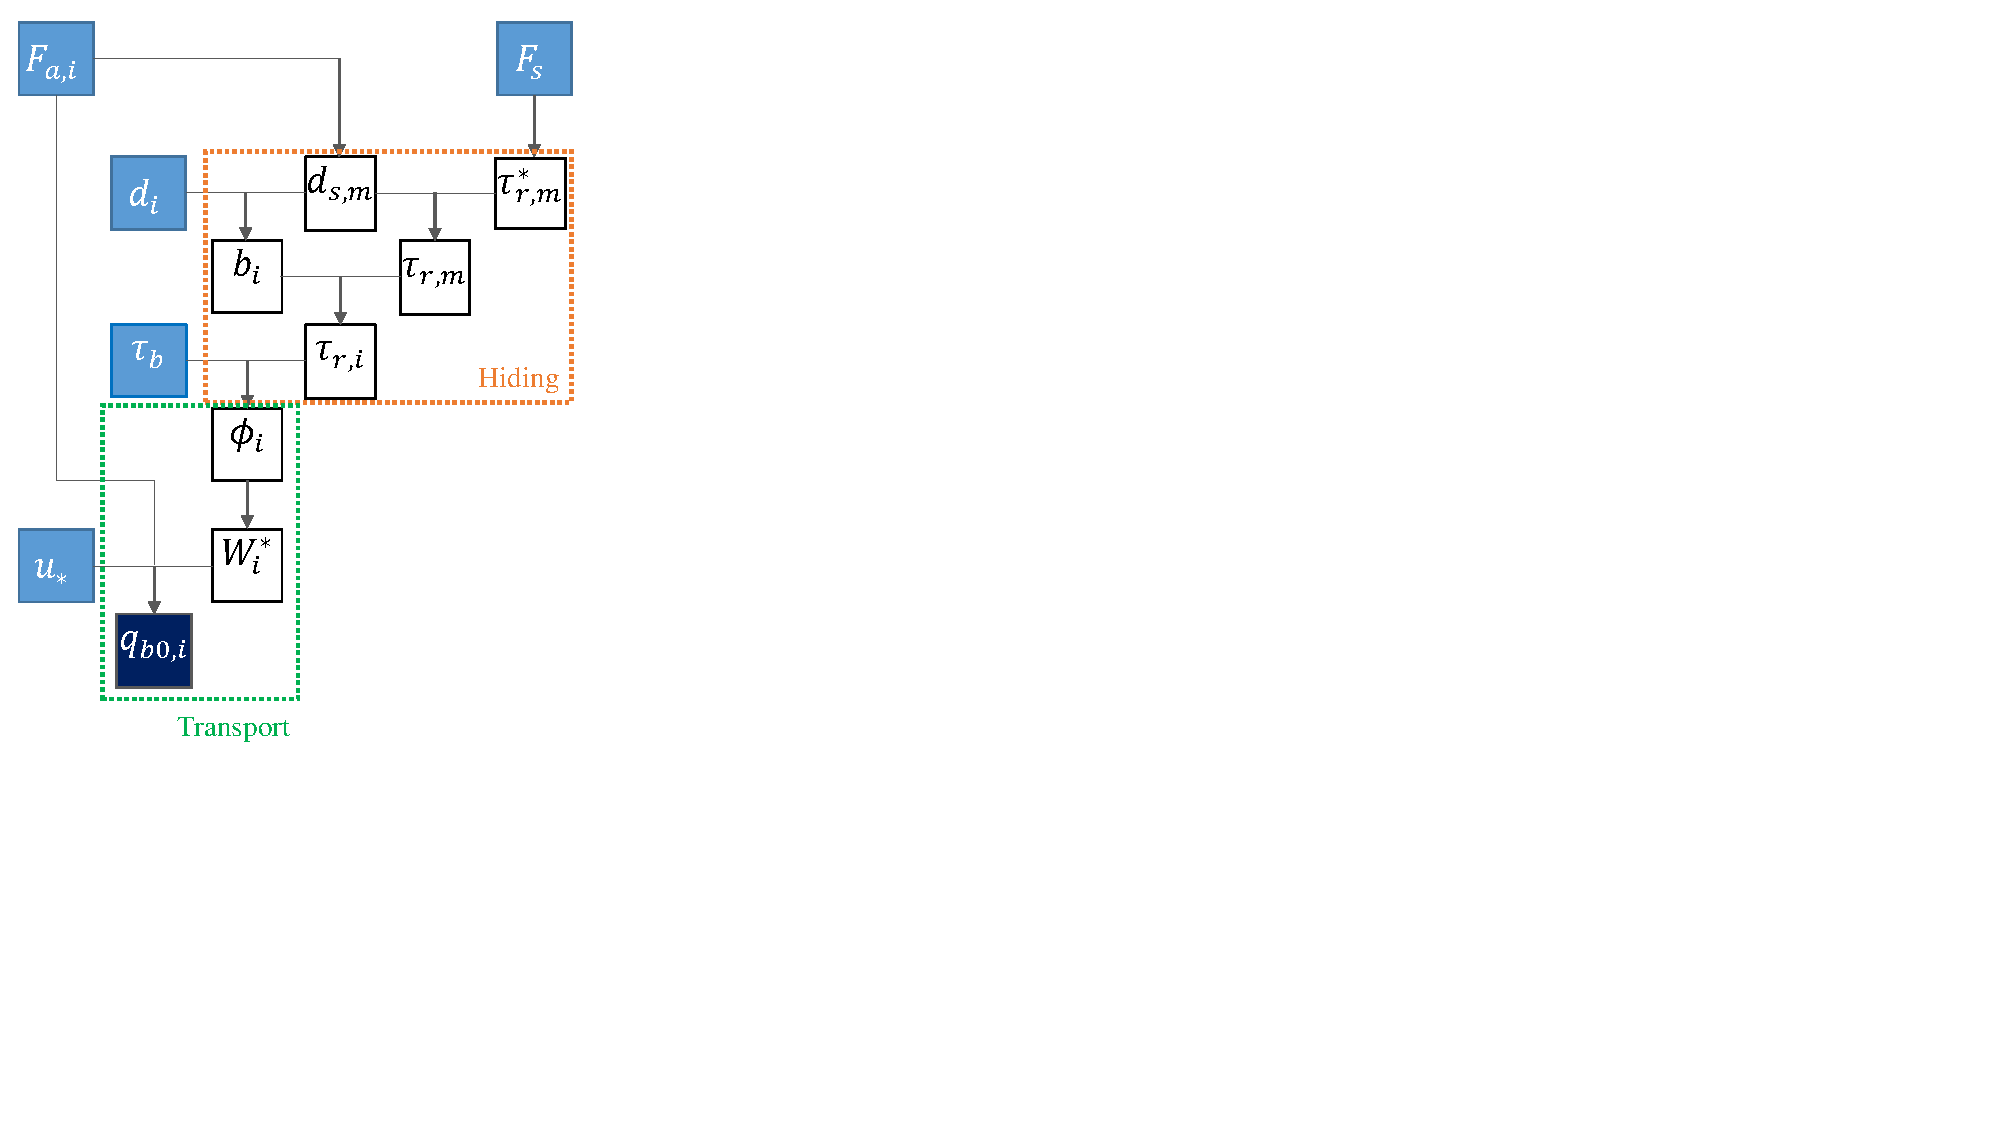
\includegraphics[width=6.5cm,trim = 0mm 60mm 220mm 0mm,clip=true]{./graphics/Wilcock_Application.pdf}
	      \caption[Scheme of application of the graded sediment transport model of WC-2003. Parameters in blue boxes are input parameters, those in white boxes are intermediary variables computed to estimate the transport rate of size fraction $i$ in the black box.]{\centering Scheme of application of the graded sediment transport model of WC-2003. Parameters in blue boxes are input parameters, those in white boxes are intermediary variables computed to estimate the transport rate of size fraction $i$ in the black box.}
	      \label{fig:Wilcock_Application}
      \end{figure}

\noindent
An exhaustive revision of some common bedload transport formulas and associated information presented in chronological order of development can be found in Table D-2 of~\cite{GarciaBook2006}.

%...............................................................................
\section{Modification of the magnitude and direction of bedload}\label{sec:corrections}
%...............................................................................
Three key aspects must be considered for computing the magnitude and direction of the bed load~\cite{Abad08}:
\begin{itemize}
\item[(a)] The effect of the local bed slope
\item[(b)] Secondary flow effects on the direction of the bed shear stress, also refered as to helical flows in the literature
\item[(c)] The bed shear stress partitioning into components affected by skin friction and drag force from bedforms
\end{itemize}
\noindent
\sisyphe{} includes methods for evaluating these three aspects.

\begin{figure}[H]%
\begin{center}
  \begin{tabular}{ccc}
    \subfloat[]{
      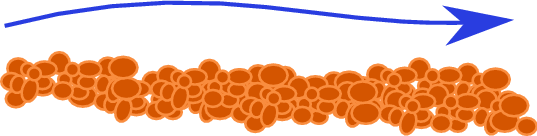
\includegraphics[scale=0.25]{./graphics/transport_1}}&
    \subfloat[]{
      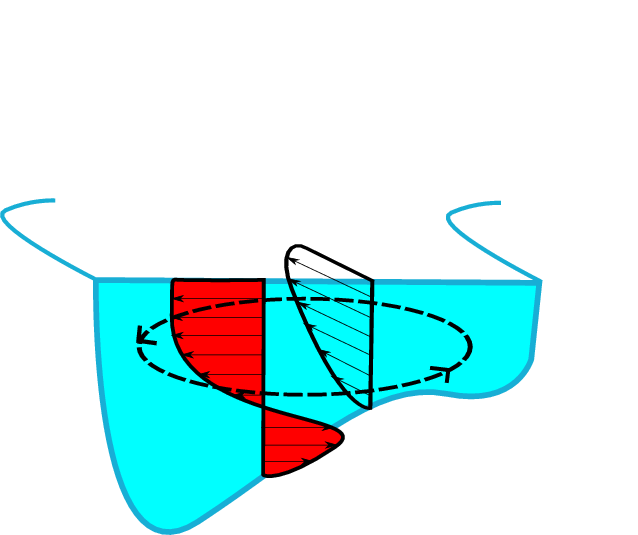
\includegraphics[scale=0.20]{./graphics/curve_4}}&
    \subfloat[]{

\includegraphics[scale=0.75]{./graphics/dunes_drag_grain}}
\end{tabular}
\end{center}
%\caption
%{ADD CAPTION\protect.}
\label{fig:ExampleImage}
\end{figure}

%-------------------------------------------------------------------------------
\subsection{Correction of the direction of the sediment transport}
%-------------------------------------------------------------------------------
The angle $\alpha$ is the angle between the sediment transport direction and the $x-$axis direction will deviate from that of the shear stress by combined action of a transverse slope and secondary currents. In a Cartesian coordinate system, the relation of van Bendegon is~\cite{}:
\begin{equation}
\displaystyle
\tan\alpha = \frac{\sin\delta-\frac{1}{f(\theta)}\frac{\partial z_b}{\partial y}}{\cos\delta-\frac{1}{f(\theta)}\frac{\partial z_b}{\partial x}}.
\end{equation}

Above, the terms $\partial z_b/\partial x$ and $\partial z_b/\partial y$ represent respectively the transverse and longitudinal slopes, $z_b$ the bottom position and $\delta$ the angle between the sediment transport vector and the flow direction, modified by spiral flow. The sediment shape function $f(\theta)$ is a function weighting the influence of the transverse bed slope, expressed as a function of the non-dimensional shear stress or Shields parameter $\theta$. It can be computed according to:

\begin{itemize}
\item Koch and Flokstra~\cite{KochFlokstra80}:
\begin{equation*}
f(\theta) = \frac{3}{2\theta}
\end{equation*}
\item Talmon \textit{et al.}~\cite{Talmon95}:
\begin{equation*}
f(\theta) = \beta_2\sqrt{\theta}
\end{equation*}
where $\beta_2$ is an empirical coefficient. In \sisyphe{} the default value is $\beta_2=0.85$, but an optimal value of $\beta_2=1.6$ was found for the calibration of numerical experiments of dunes and bars in a laboratory channel~\cite{Mendoza15}.
\end{itemize}

%-------------------------------------------------------------------------------
\subsection{Correction by secondary flow effects on the direction of the bed shear stress}
%-------------------------------------------------------------------------------
In curved channels, the direction of the sediment transport will no longer coincides with the direction of the bed shear stress,
due to the effect of the secondary flows:
\begin{equation}\label{eq:delta}
\delta = \tan^{-1}\left(\frac{v}{u}\right) - \textcolor{red}{\tan^{-1}\left(\frac{A}{r_s}h\right)} = \delta^* - \textcolor{red}{\Delta\delta},
\end{equation}
with $h$ the water depth, $(u,v)$ the components of the depth-averaged velocity field, $r_s$ the local radius of curvature and $A$ the spiral flow coefficient. Above, the term highlighted in red accounts for the effect of the spiral motion on the sediment flux. The angles $\delta^*$ and $\Delta\delta$ indicate respectively the direction of the bed shear stress (which coincides with the direction of the depth-averaged velocity) and the direction due to the effect of secondary currents.

In \sisyphe{} $A=7^*$ (Engelund's value). Nevertheless, an optimal value of $A=12$ was found for the calibration of numerical experiments of dunes and bars in a laboratory channel~\cite{Mendoza15}.

%-------------------------------------------------------------------------------
\subsection{Correction of the magnitude of the sediment transport}
%-------------------------------------------------------------------------------
The correction of the magnitude of the sediment transport proposed by Koch and Flokstra~\cite{KochFlokstra80} is based on the modification of the bed load transport rate by a factor that acts as a diffusion term in the bed evolution equation:
\begin{equation}
\begin{array}{ll} \displaystyle
Q_b^* &= Q_{b}\left(1+\beta\frac{\partial z_b}{\partial s}\right) \\
    &= Q_{b}\left[1 + \beta \left(\frac{\partial z_b}{\partial x} \cos\alpha + \frac{\partial z_b}{\partial y} \sin\alpha\right)\right],
\end{array}
\end{equation}
where $s$ is the flow direction and $\beta$ is an empirical factor accounting for the streamwise bed slope effect ($=1.3$ by default).

The correction proposed by Soulsby~\cite{Soulsby97} is based on the modification of the critical Shields parameter and is therefore only valid for threshold bedload formulas:
\begin{equation*}
\frac{\theta_{\beta cr}}{\theta_{cr}} = \frac{\cos\psi \sin\chi + 
\sqrt{\cos^2\chi \tan^2\phi - \sin^2\psi \sin^2\chi}}{\tan
\phi}
\end{equation*}
where $\theta_{\beta cr}$ is the corrected critical Shields number for a sloping bed, $\theta_{cr}$ is the critical Shields number for a flat, horizontal bed, $\phi$ is the angle of repose of the sediment, $\chi$ is the bed slope angle with the horizontal, and $\psi$ is the angle between the flow and the bed slope directions.

%-------------------------------------------------------------------------------
\section{Keywords for the modification of the intensity and direction of bed load}
%-------------------------------------------------------------------------------
The keyword \telkey{SLOPE EFFECT} (logical type variable, set to {\ttfamily = YES} by default) activates the bed slope effects. If \telkey{SLOPE EFFECT = NO}, the keywords \telkey{FORMULA FOR DEVIATION} and \telkey{FORMULA FOR SLOPE EFFECT} are not taken into account.

%-------------------------------------------------------------------------------
\subsubsection{Correction of the direction of bedload transport}
%-------------------------------------------------------------------------------
The correction of the direction of bedload transport can be done by either the Koch and Flokstra formulation \telkey{FORMULA FOR DEVIATION = 1} (integer type variable, set to {\ttfamily = 1} by default) or the Talmon et al. formulation \telkey{FORMULA FOR DEVIATION = 2}. For the latter, an associated keyword is available \telkey{PARAMETER FOR DEVIATION} (real type variable named \telkey{BETA2}, set to {\ttfamily = 0.85} by default).

%-------------------------------------------------------------------------------
\subsubsection{Correction of the intensity of bedload transport rate}
%-------------------------------------------------------------------------------
The correction of the intensity of bedload transport rate can be done by either:
\begin{itemize}
\item the Koch and Flokstra formulation \telkey{FORMULA FOR SLOPE EFFECT} (integer type variable, set to {\ttfamily = 1} by default). This keyword has the associated keyword \telkey{BETA} (real type variable, set to {\ttfamily = 1.30} by default)
\item the Soulsby formulation \telkey{FORMULA FOR SLOPE EFFECT = 2}. This keyword has the associated keyword \telkey{FRICTION ANGLE OF THE SEDIMENT} (real type variable, set to {\ttfamily = 40.} by default).
\end{itemize}

The keyword \telkey{SECONDARY CURRENTS} (logical type variable, set to {\ttfamily = NO} by default) accounts for the secondary flow correction. This keyword has the associated keyword \telkey{ SECONDARY CURRENTS ALPHA COEFFICIENT} (real type variable, set to {\ttfamily = 1.} by default) that allows the modification of the coefficient $A$ in Equation~\ref{eq:delta}. This value can be chosen as: $\rightarrow 0.75~~\text{(rough bottom)} \leq \alpha_{SC} \leq 1.0~~\text{(smooth bottom)}$. For example, if $\alpha_{SC} = 1$ then $A = 7$.

%-------------------------------------------------------------------------------
\section{Influence of the roughness on sediment transport processes}\label{sec:roug}
%-------------------------------------------------------------------------------
%-------------------------------------------------------------------------------
\subsection{Skin friction correction}\label{sec:skin}
%-------------------------------------------------------------------------------
The total bed shear stress is due to skin friction and bed form drag but \textbf{only the component due to skin friction acts on bedload}. The shear stress due to skin friction is expressed as:
\begin{equation}\label{eq:taup}
\tau'=\mu\tau_b,
\end{equation}
where $\tau_b = 0.5 \rho C_f (U^2 + V^2)$ is the total bed shear stress and $\mu$ is the friction factor:
\begin{equation}\label{eq:mu}
\mu=\frac{C_f'}{C_f}
\end{equation}
where $C_f$ is the friction coefficient due to form drag plus skin friction (specified in the hydrodynamics module), and $C_f'$ is the friction coefficient due only to skin friction, which is computed as:
\begin{equation}\label{eq:cfp}
C_f'=2\left(\frac{\kappa}{\log(12h/k_s')}\right)^2,
\end{equation}
where $\kappa$ is the von K\'arm\'an coefficient ($=0.40$), the roughness height $k_s'=\alpha_{k_s}d_{50}$, the coefficient $\alpha_{k_s}$ is a calibration parameter.

%-------------------------------------------------------------------------------
\subsection{Keywords for skin friction correction}
%-------------------------------------------------------------------------------
The keyword \telkey{SKIN FRICTION CORRECTION} (integer type variable, {\ttfamily = 1} by default) activates the correction of the bed shear stress due to skin friction:
\begin{itemize}
\item If \telkey{SKIN FRICTION CORRECTION = 0}, then $\mu=1$ and the total bed shear stress issued from the hydrodynamics computation is used
\item If \telkey{SKIN FRICTION CORRECTION = 1}, $\mu$ is computed according to Equation~\ref{eq:mu}. In this case, the friction coefficient $C_f$ is provided by the hydrodynamics steering file and $C_f'$ is computed by Equation~\ref{eq:cfp}. To compute $k_s'=\alpha_{k_s} d_{50}$, the coefficient $\alpha_{k_s}$ can be modified with the keyword \telkey{RATIO BETWEEN SKIN FRICTION AND MEAN DIAMETER} (real type variable, {\ttfamily = 3.} by default). In the numerical experiments of Mendoza \textit{et al.}~\cite{Mendoza15}, $\alpha_{k_s}=37$ for dunes and $\alpha_{k_s}=3.6$ for bars.  

 \begin{WarningBlock}{Note:}
  By default, the keyword \telkey{SKIN FRICTION CORRECTION = 1}. In the presence of very shallow waters, this correction can present stability issues. For this case, we suggest the user to set the keyword \telkey{SKIN FRICTION CORRECTION = 0}.
  \end{WarningBlock}

\item If \telkey{SKIN FRICTION CORRECTION = 2}, the presence of ripples is taken into account to compute $\mu$ (see subroutine \texttt{tob\_sisyphe.f}). For this option, a bedform predictor is used to calculate the bedform roughness $k_r$ in order to account for the effect of ripples. Both $k_r$
and $k_s'$ should influence the transport rates. It is assumed that:
\begin{equation}\label{eq:mu2}
\mu =\frac{C_f'^{0.75} C_r^{0.25}}{C_f}, 
\end{equation}
where the quadratic friction $C_r$ due to bedforms is calculated as a
function of $k_r$ (see \S~\ref{sec:bedroughpredictor}). 
\end{itemize}

%-------------------------------------------------------------------------------
\subsection{Bed roughness predictor}\label{sec:bedroughpredictor}
%-------------------------------------------------------------------------------
A natural sediment bed is generally covered with bedforms, with length $\lambda_d$ (m)
and height $\eta_d$ (m). The presence of bed forms greatly modifies the boundary
layer flow structure, with the formation of recirculation cells and
depressions in the lee of bedforms.\\

Depending on the flow and sediment transport rates, the size of bed
forms ranges from a few centimeters for ripples to a few tens of meter for
mega-ripples. The dimension of dunes scales with the water depth $h$, such that $\eta_d
\approx 0.4 h$ and  $\lambda_d\approx [6-10] h$.\\

In most cases, large scale models do not resolve the small to medium
scale bedforms (such as ripples or mega-ripples) which need therefore to be parameterized by increasing the friction coefficient. To determine bed roughness, there are two options available in \sisyphe{}:
\begin{itemize}
\item By imposing the friction coefficient based on friction laws: in this case the values of the friction coefficients are provided by \telemac{2D} or \telemac{3D}.
\item By predicting the value of the bed roughness as a function of flow and sediment parameters using a bed roughness predictor. This option is discussed below.
\end{itemize}
Different options are programmed in \sisyphe to predict the total bed
roughness through the associated keywords \telkey{BED ROUGHNESS PREDICTION} and \telkey{BED ROUGHNESS PREDICTOR OPTION}. It is recalled that the bed friction option of \sisyphe is not
used in the case of internal coupling with \telemac{2D} or \telemac{3D}.
\begin{itemize}
\item For {\ttfamily BED ROUGHNESS PREDICTOR OPTION = 1}: the bed is assumed to be flat $k_s = k_s'= \alpha_{k_s} d_{50}$, with $\alpha_{k_s}$ a constant (assumed to be equal to $3.$), modified by the keyword \telkey{RATIO BETWEEN SKIN FRICTION AND MEAN DIAMETER}. 
\item {\ttfamily BED ROUGHNESS PREDICTOR OPTION = 2}: the bed is assumed to be covered by ripples.
  \begin{itemize}
    \item For currents only, the ripple bed roughness is function of the mobility number, see~\cite{vanRijn07}:
\begin{equation*}
k_r =\left\{\begin{array}{ll}
d_{50}(85-65\tanh(0.015(\Psi-150))) & \text{for\,} \Psi<250\\
20 d_{50} & \text{otherwise} 
\end{array}
\right.
\end{equation*}
with $\Psi =U^2/(s-1)gd_{50}$.

    \item For waves and combined waves and currents, bedform dimensions are calculated
as a function of wave parameters following the method of Wiberg and Harris~\cite{WibergHarris}. 
The wave-induced bedform bed roughness $k_r$ is calculated as a function of the wave-induced bedform 
height $\eta_r$: 
\begin{equation}
k_r = \max(k_s', \eta_r).
\end{equation}
Then $k_s=k_s'+k_r$.
  \end{itemize}
 
\item {\ttfamily IKS = 3}: for currents only, the van Rijn's total bed roughness predictor~\cite{vanRijn07, Huybrechts} has been implemented. 
The total bed roughness can be decomposed into a grain
roughness $k_s'$, a small-scale ripple roughness $k_r$, a mega-ripple 
component $k_{mr}$, and a dune roughness $k_d$:
\begin{equation}\label{eq:totalbedroughness}
k_s = k_s' + \sqrt{k_r^2 + k_{mr}^2 + k_d^2}. 
\end{equation}
Both small scale ripples and grain roughness have an influence on the
sediment transport laws, while the mega-ripples and dune roughness only
contribute to the hydrodynamic model (total friction). In Equation~\ref{eq:totalbedroughness}, the general expression for megaripples roughness $k_{mr}$ is given by:
\begin{equation}
k_{mr} = 0.00002\,f_{ts}\,h\,(1-\exp^{-0.05\Psi})\,(550-\Psi),
\end{equation}
with
\begin{equation*}
f_{ts} =\left\{\begin{array}{ll}
d_{50}/(1.5d_{sand}) & \text{for\,} d_{50}\leq 1.5d_{sand}\\
1.0 & \text{otherwise} 
\end{array}
\right.
\end{equation*}
and the general expression for dune roughness $k_d=0.00008\,f_{ts}\,h\,(1-\exp^{-0.02\Psi})\,(600-\Psi)$.

\end{itemize}

%-------------------------------------------------------------------------------
\section{Boundary conditions for bedload}
%-------------------------------------------------------------------------------
The specification of boundary conditions is done in a boundary condition file, usually named with extension \texttt{*.cli}. The reader is referred to \S\ref{sec:flags} for the definition of the different flags used in the boundary condition file.

\subsection{Wall boundary conditions}
At banks and islands, the bedload transport rate is set to zero. For this case, the flag \texttt{LIEBOR} is set \texttt{= 2} as shown in the example below:

\begin{lstlisting}[frame=trBL]
2 2 2 0.0 0.0 0.0 0.0 (*@\color{PantoneRed}2@*) 0.0 0.0 0.0 565 1
\end{lstlisting}

\subsection{Inflow boundary conditions}
In a depth-averaged 2D sediment transport model, the sediment discharge must be given at each point of the inflow boundary. The different cases can be present:
\subsubsection{Equilibrium sediment discharge}
For this case, the flag \texttt{LIEBOR} is set \texttt{= 5} and the flag \texttt{EBOR} is set \texttt{= 0.0} (no bottom change at the inflow boundary) as shown in the example below:

\begin{lstlisting}[frame=trBL]
4 5 5 0.0 0.0 0.0 0.0 (*@\color{PantoneRed}5@*) (*@\color{PantoneRed}0.0@*) 0.0 0.0 565 1
\end{lstlisting}

\subsubsection{Constant sediment discharge}
For this case, boundary condition files are needed for both \telemac{2D} and \sisyphe{}. In the \sisyphe{}'s boundary condition file, the flag \texttt{LIQBOR = 5} and \texttt{LIEBOR = 4}. The imposed solid discharge can be specified as follows:
\begin{itemize}
\item A value of the unit solid discharge [m$^2$/s] in the column \texttt{Q2BOR} of the \sisyphe{}'s boundary condition file, as shown in the example below for an imposed unit discharge \texttt{Q2BOR=}$1.0$m$^2$/s:
\begin{lstlisting}[frame=trBL]
4 (*@\color{PantoneRed}5@*) 5 (*@\color{PantoneRed}1.0@*) 0.0 0.0 0.0 (*@\color{PantoneRed}4@*) 0.0 0.0 0.0 565 1
\end{lstlisting}

Particular cases of \texttt{Q2BOR} can be programmed in the subroutine \texttt{conlit.f}.
  
\item A value of the total solid discharge (without pores) [m$^3$/s] given through the keyword \telkey{PRESCRIBED SOLID DISCHARGES} (sequence of real values separated by semi-colons, one value per liquid boundary, no default value) in the steering file, as shown in the example below for an imposed total discharge equal to $1.0$m$^3$/s:
\begin{lstlisting}[frame=trBL]
4 (*@\color{PantoneRed}5@*) 5 0.0 0.0 0.0 0.0 (*@\color{PantoneRed}4@*) 0.0 0.0 0.0 565 1
\end{lstlisting}

\begin{lstlisting}[frame=trBL]
PRESCRIBED SOLID DISCHARGES : 1.0
\end{lstlisting}
 
\end{itemize}

\subsubsection{Time-series of sediment discharge}
Time-series values of sediment discharge are specified in a file through the keyword \telkey{LIQUID BOUNDARIES FILE} (character type). The \sisyphe{}'s boundary condition file must contain the flags as shown below:
\begin{lstlisting}[frame=trBL]
4 (*@\color{PantoneRed}5@*) 5 0.0 0.0 0.0 0.0 (*@\color{PantoneRed}4@*) 0.0 0.0 0.0 565 1
\end{lstlisting}

The keyword \telkey{PRESCRIBED SOLID DISCHARGES} must be also included in the steering file, with an arbitrary value.

\subsection{Outflow boundary conditions}
At the outflow boundary, bedload does not require any particular boundary condition.
For this case, the flag \texttt{LIEBOR} is set \texttt{= 4} as shown in the example below:

\begin{lstlisting}[frame=trBL]
5 4 4 0.0 0.0 0.0 0.0 (*@\color{PantoneRed}4@*) 0.0 0.0 0.0 565 1
\end{lstlisting}

\begin{WarningBlock}{Note:}
When the keyword \telkey{PRESCRIBED SOLID DISCHARGES} is used, the mass balance provided in the listing printouts information accounts for the pores $=Q_b/(1-\lambda)$, with $\lambda$ the porosity.
\end{WarningBlock}

%-------------------------------------------------------------------------------
\section{Numerical treatments}
%-------------------------------------------------------------------------------
\subsection{Rigid beds}
Non-erodable beds are treated numerically by limiting the bed erosion and letting incoming sediment pass over. The problem of rigid beds is conceptually trivial but numerically complex. 

For finite elements the minimum water depth algorithm allows a natural treatment of rigid
beds, see~\cite{Hervouet11}. The sediment is managed as a layer with a
depth that must remain positive, and the Exner equation is solved similarly to the shallow water continuity equation in the subroutine {\ttfamily positive\_depths.f} of the \textsc{Bief} library.

The space location and position of the rigid bed can be modified in the subroutine \texttt{noerod.f}. By default, the position of the rigid bed is located at $z=-100$m.

\subsection{Tidal flats}
Tidal flats are areas of the computational domain where the water depth can become zero during the simulation. For finite elements the minimum water depth algorithm allows a natural treatment of tidal flats, see~\cite{Hervouet11} and the Exner equation is solved similarly to the shallow water continuity equation in the subroutine {\ttfamily positive\_depths.f} of the \textsc{Bief} library.

Improvements of the numerical results where wetting and drying processes are present can be achieved by using the keyword \telkey{MINIMUM DEPTH FOR BEDLOAD} (real type variable, set to {\ttfamily = 1.E-2}m by default), which cancels sediment fluxes to and from dry points.  

The default value can be modified by the user. As a guideline, we can suggest a value in the range $[2-3]\times d_{50}$, being $d_{50}$ the median sediment diameter.

A complete treatment of tidal flats is given in the \telemac{2D} users manual.


%-------------------------------------------------------------------------------
\subsection{Morphological factor}
%-------------------------------------------------------------------------------
The morphological factor, keyword \telkey{MORPHOLOGICAL FACTOR} (real type, set to {\ttfamily = 1.0} by default), increases the bottom change rates with a constant factor $N$. The new bed level represents a simulation period of $N$ hydrodynamic time steps. For example, using $1$ semi-diurnal tide ($\approx$12 hours) and a morphological factor of $10$ will result in an actual simulated time period of $120$ hours.

In theory, assuming that the morphodynamic changes are small compared to the hydrodynamic changes, 
this approach reduces the computational effort without significant loss of model quality. Further details can be found in~\cite{Knaapen12} and references therein.

%-------------------------------------------------------------------------------
\subsection{Sediment Slide}
%-------------------------------------------------------------------------------
An iterative algorithm prevents the bed slope to become greater than the maximum friction angle ($\theta_s \approx 32^\circ-40^\circ$). A rotation of each element is then performed in order to insure: \textit{(i)} mass continuity and \textit{(ii)} bed slope $<$ friction angle: $|\Grad(z_b)| < \tan(\theta_s)$. The subroutine \texttt{maxslope.f} was recently modified to avoid stability issues by controlling the amount of sediment that slides. This quantity was set at 10\% of the quantity needed to achieve the required slopes, therefore slowing down the slope correction.\\

This option is activated by the keyword \texttt{SEDIMENT SLIDE = YES} (logical type variable, set to {\ttfamily = NO} by default). The friction angle can be modified with the keyword {\ttfamily FRICTION ANGLE OF SEDIMENT} (real type variable, {\ttfamily = 40.} by default). Further details can be found in~\cite{ElKadiAbderrezzak201675}.



\pagebreak

%-------------------------------------------------------------------------------
\section{Useful graphical printouts for bedload}
%-------------------------------------------------------------------------------
Through the keyword \telkey{ VARIABLES FOR GRAPHIC PRINTOUTS}, some useful printouts for bedload sediment transport are listed below:
\begin{lstlisting}[frame=trBL]  
TOB="Bed shear stress(N/m2)";
MU ="Skin friction coefficient";
M="bed-load discharge (m2/s)";
N="bed-load discharge along x axis (m2/s)";
P="bed-load discharge along y axis (m2/s)";
E="bottom evolution (m)";
QSBL="bed load transport rate (m2/s)";
\end{lstlisting}

\begin{WarningBlock}{Note:}
The sediment discharge is the mass of sedimentary material, both particulate and dissolved, that passes across a given flow-transverse cross section of a given flow in unit time. The flag {\ttfamily M} accounts for the total solid discharge (bed load and suspended load), while {\ttfamily QSBL} accounts for the bed load solid discharge.
\end{WarningBlock}

